%\documentclass[handout]{beamer}
\documentclass[ignorenonframetext]{beamer}
\usepackage{textpos}
\usepackage{graphicx}
\usepackage{pgf}
\usepackage{caption}
\usepackage{listings}
\usepackage{multimedia}
\usepackage{gensymb}
\usepackage{amsmath, mathrsfs}
\usepackage[fixed]{fontawesome5}
\usepackage{tcolorbox}
\usepackage{tikz}
\usepackage{xcolor}
\tcbuselibrary{skins,raster}
\usetikzlibrary{positioning,fit,calc,decorations.pathmorphing,backgrounds}

% Swagger UI method colors
\definecolor{swagger-get}{HTML}{61AFFE}
\definecolor{swagger-post}{HTML}{49CC90}
\definecolor{swagger-put}{HTML}{FCA130}
\definecolor{swagger-delete}{HTML}{F93E3E}

% \captionsetup[figure]{labelformat=empty}% redefines the caption setup of the figures environment in the beamer class.

\lstdefinestyle{yaml}{
     basicstyle=\ttfamily\color{blue}\tiny,
     rulecolor=\color{black},
     string=[s]{'}{'},
     stringstyle=\color{blue},
     comment=[l]{:},
     commentstyle=\color{black},
     morecomment=[l]{-}
 }

\usetheme{Boadilla}
\usefonttheme{serif}
% \mode<presentation>
% {
%  \usefonttheme{serif}
% % \useoutertheme{sidebar}
% %   \logo{
\includegraphics[height=1cm]{elec_logo.pdf}}
% }

\title[TART API]{The TART API}

\author[Scheel]{Max Scheel}

\institute[Elec Research]
{
  Electronics Research Foundation \\
  New Zealand \\
  \vspace{2cm}
  
\includegraphics[width=0.6\linewidth]{../tart_overview/fig/elec_header_font.pdf}
}

\logo{\pgfputat{\pgfxy(-0.72,7.7)}{\pgfbox[center,base]{
\includegraphics[width=1cm]{../tart_overview/fig/elec_logo.pdf}}}}

\date[TART Madagascar 2026] % (optional, should be abbreviation of conference name)
{}

% \addtobeamertemplate{headline}{}{%
% \begin{textblock*}{100mm}(0.87\textwidth,2mm)
% 
\includegraphics[height=1.5cm]{elec_logo.pdf}
% \end{textblock*}}

\begin{document}

% Abstract: In this talk I'll give an overview of Africa's newest radio telescope, the TART, recently installed in Mauritius in a joint effort between SARAO, the University of Otago (NZ). I'll talk about TARTs origins, it's design and open-source philosophy as well as the upcoming project to install TART telescopes in the SKA African partner nations. I'll also include some details about improvements that will appear in TART-3, the next version of TART!

\begin{frame}
	\titlepage
\end{frame}

\begin{frame}{Outline}
	\begin{enumerate}
		\item \textbf{Introduction} --- What is the TART API and why?
		\item \textbf{System Architecture} --- Network, telescopes, services
		\item \textbf{RESTful API Basics} --- HTTP methods, JSON, stateless
		\item \textbf{The TART API in Practice} --- Endpoints, examples
		\item \textbf{API in the Age of AI} --- Agents, composability, safety
		\item \textbf{Single Telescope Node} --- Hardware to software stack
		\item \textbf{Summary \& Discussion}
	\end{enumerate}
\end{frame}

\section{Introduction}

\begin{frame}{Introduction}
	\begin{itemize}
		\item TART = Transient Array Radio Telescope
		\item 10+ telescopes deployed across Africa, Asia, NZ
		\item Each telescope runs a \textbf{RESTful API}
		\item All telescopes accessible via a single gateway:\\
		      {\small\url{https://api.elec.ac.nz/}}
		\item This talk: how the API works, how to use it, and why it matters
	\end{itemize}
\end{frame}

\section{RESTful API Basics}

\begin{frame}{What is a RESTful API?}
	\begin{itemize}
		\item \textbf{REST} = Representational State Transfer
		\item Stateless client--server communication over HTTP
		\item Standard HTTP methods:
		      \begin{description}
			      \item[GET] Retrieve data
			      \item[POST] Create / submit data
			      \item[PUT] Update existing resource
			      \item[DELETE] Remove a resource
		      \end{description}
		\item Resources identified by URLs
		\item Data exchanged as \textbf{JSON}
		\item No session state on the server --- each request is self-contained
	\end{itemize}

	\vspace{0.3cm}
	{\small Example:}\\
	\texttt{GET https://api.elec.ac.nz/tart/mu-udm/api/v1/imaging/vis}\\
	{\scriptsize $\rightarrow$ returns latest visibilities as JSON}
\end{frame}

\begin{frame}[fragile]{RESTful API Example}
	{\small Request:}
	\begin{lstlisting}[basicstyle=\ttfamily\scriptsize\color{white}, backgroundcolor=\color{black!85}, rulecolor=\color{black!50}, frame=single, framesep=0.4em, xleftmargin=0.5em, xrightmargin=0.5em]
curl -X 'GET' \
  'https://api.elec.ac.nz/tart/ghana/api/v1/info' \
  -H 'accept: application/json'
	\end{lstlisting}

	\vspace{0.2cm}
	{\small Response:}
	\begin{lstlisting}[basicstyle=\ttfamily\scriptsize\color{black!85}, backgroundcolor=\color{gray!8}, rulecolor=\color{gray!40}, frame=single, framesep=0.4em, xleftmargin=0.5em, xrightmargin=0.5em]
{
  "info": {
    "name": "GRAO - Ghana",
    "operating_frequency": 1575420000,
    "L0_frequency": 1571328000,
    "baseband_frequency": 4092000,
    "sampling_frequency": 16368000,
    "bandwidth": 2500000,
    "num_antenna": 24,
    "location": {
      "lon": -0.305557,
      "lat": 5.749725,
      "alt": 72
    }
  }
}
	\end{lstlisting}
\end{frame}

\begin{frame}{Why an API Spec Matters --- in the Age of AI}
	\textbf{A well-defined API is a contract --- for humans \emph{and} machines.}

	\vspace{0.3cm}
	\begin{itemize}
		\item \textbf{AI agents can operate the telescope}
		      \begin{itemize}
			      \item LLMs read OpenAPI specs natively
			      \item Autonomous calibration, monitoring, scheduling
		      \end{itemize}
		\item \textbf{Composability}
		      \begin{itemize}
			      \item Chain tools: observe $\rightarrow$ calibrate $\rightarrow$ image $\rightarrow$ publish
			      \item Integrate with any language / platform
		      \end{itemize}
		\item \textbf{Reproducibility}
		      \begin{itemize}
			      \item Every action is a URL + JSON --- fully logged, replayable
			      \item No hidden GUI state
		      \end{itemize}
		\item \textbf{Validation \& safety}
		      \begin{itemize}
			      \item Schema enforces types, ranges, required fields
			      \item Auth separates read (public) from write (protected)
		      \end{itemize}
		\item \textbf{Auto-generated clients \& docs}
		      \begin{itemize}
			      \item SDKs in Python, JS, etc.\ from the spec
			      \item Documentation is always up-to-date
		      \end{itemize}
	\end{itemize}
\end{frame}

\begin{frame}[fragile]{API Documentation --- OpenAPI / Swagger}
	\begin{itemize}
		\item The TART API follows the \textbf{OpenAPI} specification
		\item Interactive Swagger UI at: {\small \url{https://api.elec.ac.nz/docs/}}
	\end{itemize}

	\vspace{0.2cm}
	\textbf{API route groups:}
	{\scriptsize
		\colorbox{swagger-get!15}{\textbf{\textcolor{swagger-get}{GET}}} public \quad
		\colorbox{swagger-post!15}{\textbf{\textcolor{swagger-post}{POST}}} auth required \quad
		\colorbox{swagger-put!15}{\textbf{\textcolor{swagger-put}{PUT}}} auth required
	}

	\vspace{0.1cm}
	{\small\ttfamily
		\begin{tabular}{@{}l l l@{}}
			\textbf{authentication} & \colorbox{swagger-post!15}{\textcolor{swagger-post}{POST}} & /auth, /auth/refresh                      \\
			\textbf{status}         & \colorbox{swagger-get!15}{\textcolor{swagger-get}{GET}}    & /status/fpga, /status/channel             \\
			\textbf{operation}      & \colorbox{swagger-get!15}{\textcolor{swagger-get}{GET}}    & /mode, /mode/current                      \\
			                        & \colorbox{swagger-post!15}{\textcolor{swagger-post}{POST}} & /mode/\{mode\}, /loop/\{mode\}            \\
			\textbf{info}           & \colorbox{swagger-get!15}{\textcolor{swagger-get}{GET}}    & /info                                     \\
			\textbf{imaging}        & \colorbox{swagger-get!15}{\textcolor{swagger-get}{GET}}    & /imaging/vis, /imaging/antenna\_positions \\
			\textbf{calibration}    & \colorbox{swagger-get!15}{\textcolor{swagger-get}{GET}}    & /calibration/gain                         \\
			                        & \colorbox{swagger-post!15}{\textcolor{swagger-post}{POST}} & /calibration/gain, .../antenna\_positions \\
			\textbf{acquisition}    & \colorbox{swagger-get!15}{\textcolor{swagger-get}{GET}}    & /acquire/\{raw,vis\}/save                 \\
			                        & \colorbox{swagger-put!15}{\textcolor{swagger-put}{PUT}}    & /acquire/\{raw,vis\}/save/\{flag\}        \\
			                        & \colorbox{swagger-put!15}{\textcolor{swagger-put}{PUT}}    & /acquire/.../num\_samples\_exp/\{exp\}    \\
			\textbf{data}           & \colorbox{swagger-get!15}{\textcolor{swagger-get}{GET}}    & /raw/data, /vis/data                      \\
		\end{tabular}
	}
\end{frame}

\begin{frame}[fragile]{API Example --- Visibility Data}
	{\small Request:}
	\begin{lstlisting}[basicstyle=\ttfamily\scriptsize\color{white}, backgroundcolor=\color{black!85}, rulecolor=\color{black!50}, frame=single, framesep=0.4em, xleftmargin=0.5em, xrightmargin=0.5em]
curl -X 'GET' \
  'https://api.elec.ac.nz/tart/ghana/api/v1/vis/data' \
  -H 'accept: application/json'
	\end{lstlisting}

	\vspace{0.2cm}
	{\small Response (handles to vis \& raw HDF5 files):}
	\begin{lstlisting}[basicstyle=\ttfamily\scriptsize\color{black!85}, backgroundcolor=\color{gray!8}, rulecolor=\color{gray!40}, frame=single, framesep=0.4em, xleftmargin=0.5em, xrightmargin=0.5em]
[
  {
    "filename": "vis/vis_2026-06-02_11_29_39.hdf",
    "checksum": "509f48d30a83a791...4e470bf",
    "timestamp": "2026-06-02T11:29:39.510412+00:00"
  },
  ...
]
	\end{lstlisting}
\end{frame}

\begin{frame}[fragile]{API Example --- Acquisition Parameters}
	{\small Number of samples = $2^N$ (exponent $N \in [16, 24]$):}

	\vspace{0.3cm}
	{\small Read current setting:}
	\begin{lstlisting}[basicstyle=\ttfamily\scriptsize\color{white}, backgroundcolor=\color{black!85}, rulecolor=\color{black!50}, frame=single, framesep=0.4em, xleftmargin=0.5em, xrightmargin=0.5em]
curl -X 'GET' '.../api/v1/acquire/vis/num_samples_exp'
	\end{lstlisting}
	\begin{lstlisting}[basicstyle=\ttfamily\scriptsize\color{black!85}, backgroundcolor=\color{gray!8}, rulecolor=\color{gray!40}, frame=single, framesep=0.4em, xleftmargin=0.5em, xrightmargin=0.5em]
{"N_samples_exp": 20}  // 2^20 = 1048576 samples
	\end{lstlisting}

	\vspace{0.3cm}
	{\small Update setting (requires auth):}
	\begin{lstlisting}[basicstyle=\ttfamily\scriptsize\color{white}, backgroundcolor=\color{black!85}, rulecolor=\color{black!50}, frame=single, framesep=0.4em, xleftmargin=0.5em, xrightmargin=0.5em]
curl -X 'PUT' '.../api/v1/acquire/vis/num_samples_exp/22' \
  -H 'Authorization: Bearer <token>'
	\end{lstlisting}
	\begin{lstlisting}[basicstyle=\ttfamily\scriptsize\color{black!85}, backgroundcolor=\color{gray!8}, rulecolor=\color{gray!40}, frame=single, framesep=0.4em, xleftmargin=0.5em, xrightmargin=0.5em]
{"N_samples_exp": 22}  // 2^22 = 4194304 samples
	\end{lstlisting}
\end{frame}

\begin{frame}{Reference URL}
	\url{https://tart.elec.ac.nz/docs/basics/tart-api/}
\end{frame}

\section{Summary}

\begin{frame}{Summary}
	\begin{itemize}
		\item TART telescopes are fully controlled via a \textbf{RESTful API}
		\item 10+ telescopes connected through \textbf{Headscale/WireGuard} VPN
		\item Single gateway at \texttt{api.elec.ac.nz} proxies to all nodes
		\item OpenAPI spec $\rightarrow$ auto-docs, validation, AI-ready
		\item Public \colorbox{swagger-get!15}{\textcolor{swagger-get}{GET}} endpoints for data access
		\item Protected \colorbox{swagger-put!15}{\textcolor{swagger-put}{PUT}}/\colorbox{swagger-post!15}{\textcolor{swagger-post}{POST}} for telescope control
	\end{itemize}

	\vspace{0.4cm}
	\centering
	\begin{tabular}{ll}
		\textbf{API Gateway:}   & \url{https://api.elec.ac.nz/}       \\
		\textbf{Swagger Docs:}  & \url{https://api.elec.ac.nz/docs/}  \\
		\textbf{Telescope Map:} & \url{https://map.elec.ac.nz/}       \\
		\textbf{Documentation:} & \url{https://tart.elec.ac.nz/docs/} \\
	\end{tabular}
\end{frame}

\section{System Architecture}

\begin{frame}{TART Network Architecture}
	\centering
	\begin{tikzpicture}[
			node distance=0.5cm and 0.8cm,
			every node/.style={font=\scriptsize},
			tartbox/.style={draw=orange!70, rounded corners, fill=orange!5,
					inner sep=0.2em, line width=0.06em, minimum width=1.6cm, align=center, font=\tiny},
			serverbox/.style={draw=blue!60, rounded corners, fill=blue!5,
					inner sep=0.3em, line width=0.08em, minimum width=2.2cm, align=center, font=\scriptsize},
			servicebox/.style={draw=blue!40, rounded corners, fill=white,
					inner sep=0.2em, line width=0.05em, minimum width=1.8cm, align=center, font=\tiny},
			clientbox/.style={draw=green!60!black, rounded corners, fill=green!5,
					inner sep=0.2em, line width=0.06em, minimum width=1.4cm, align=center, font=\tiny},
			wg/.style={<->, >=stealth, line width=0.08em, draw=purple!70, dashed},
			conn/.style={->, >=stealth, line width=0.08em, draw=black!60},
		]

		% --- nginx at top (with tailscale sidecar inside) ---
		\node[serverbox, minimum height=1.5cm] (nginx) {
			\faIcon{server}~\textbf{nginx}\\[-1pt]
			api.elec.ac.nz\\[2pt]
			{\tiny\color{purple!70}\faIcon{network-wired} tailscale}
		};
		% Public interface label
		\node[font=\tiny, text=green!50!black, right=0.1cm of nginx.east, anchor=west] (pub-side) {Public};

		% Headscale below
		\node[servicebox, below=0.6cm of nginx, draw=purple!50, fill=purple!5] (headscale) {
			\faIcon{network-wired}~\textbf{Headscale}
		};

		% nginx (via tailscale) connects to headscale
		\draw[wg] (nginx.south) -- (headscale.north);
		% map.elec.ac.nz below headscale (has its own nginx + API)
		\node[servicebox, below=0.8cm of headscale, minimum width=2.2cm] (mapui) {
			\faIcon{map}~\textbf{map.elec.ac.nz}\\[-1pt]
			{\tiny API + nginx}
		};

		% gRPC: map API -> headscale
		\draw[conn, <->, draw=purple!60, dashed] (mapui) -- node[right, font=\tiny, text=purple!60] {gRPC} (headscale);

		% --- Telescopes (left, fanning into headscale) ---
		\node[tartbox, left=2.5cm of headscale, yshift=1.2cm] (tart1) {\faIcon{broadcast-tower} nz-sig};
		\node[tartbox, left=2.5cm of headscale, yshift=0.4cm] (tart2) {\faIcon{broadcast-tower} za-kat};
		\node[tartbox, left=2.5cm of headscale, yshift=-0.4cm] (tart3) {\faIcon{broadcast-tower} mu-udm};
		\node[left=2.5cm of headscale, yshift=-1.0cm, font=\scriptsize] (dots) {\vdots};
		\node[tartbox, left=2.5cm of headscale, yshift=-1.5cm] (tartn) {\faIcon{broadcast-tower} bd-iub};
		\node[font=\tiny, text=orange!70, above=0.1cm of tart1, align=center] {Telescopes\\Tailscale clients};

		% --- Clients (right, fanning out from nginx) ---
		\node[clientbox, right=2.5cm of nginx] (python) {\faIcon{python} tart\_tools};
		\node[clientbox, right=2.5cm of nginx, yshift=-0.8cm] (cli) {\faIcon{terminal} curl};
		\node[clientbox, right=2.5cm of nginx, yshift=-1.6cm] (browser) {\faIcon{laptop} Browser};

		% --- WireGuard connections (all fan into Headscale) ---
		\draw[wg] (tart1.east) -- (headscale.west);
		\draw[wg] (tart2.east) -- (headscale.west);
		\draw[wg] (tart3.east) -- (headscale.west);
		\draw[wg] (tartn.east) -- (headscale.west);
		\node[font=\tiny\bfseries, text=purple!70, above=0.15cm of tart1.north east, anchor=south west] {WireGuard};

		% --- Client connections (fan out from Public side) ---
		\draw[conn] (nginx.east) -- (python.west);
		\draw[conn] (nginx.east) -- (cli.west);
		\draw[conn] (nginx.east) -- (browser.west);
		\node[font=\tiny\bfseries, text=green!50!black, above=0.05cm of python.north west, anchor=south east] {HTTPS};

		% --- map.elec.ac.nz serves the UI to Browser ---
		\draw[conn] (mapui.east) -- (browser.west)
		node[below, midway, font=\tiny, text=blue!50] {UI};

		% --- Example URL ---
		\node[below=0.4cm of mapui, font=\tiny, text=black!50] {
			\texttt{api.elec.ac.nz/tart/mu-udm/api/v1/imaging/vis}
		};

	\end{tikzpicture}
\end{frame}

\section{Single Telescope Node}

\begin{frame}{Single Telescope Node}
	\centering
	\begin{tikzpicture}[
			node distance=0.4cm and 0.8cm,
			every node/.style={font=\scriptsize},
			hwbox/.style={draw=orange!70, rounded corners, fill=orange!5,
					inner sep=0.2em, line width=0.06em, minimum width=1.4cm, align=center, font=\tiny},
			container/.style={draw=blue!50, rounded corners, fill=blue!5,
					inner sep=0.2em, line width=0.06em, minimum width=2.0cm, align=center, font=\tiny},
			clientbox/.style={draw=green!60!black, rounded corners, fill=green!5,
					inner sep=0.2em, line width=0.06em, minimum width=1.6cm, align=center, font=\tiny},
			cloudbox/.style={draw=blue!60, rounded corners, fill=blue!5,
					inner sep=0.2em, line width=0.06em, minimum width=1.8cm, align=center, font=\tiny},
			nodebox/.style={draw=black!40, rounded corners=0.3cm, fill=yellow!3,
					inner sep=0.4em, line width=0.06em},
			dockerbox/.style={draw=cyan!60, rounded corners=0.2cm, fill=cyan!3,
					inner sep=0.4em, line width=0.06em},
			conn/.style={->, >=stealth, line width=0.08em, draw=black!60},
			wg/.style={<->, >=stealth, line width=0.08em, draw=purple!70, dashed},
		]

		% --- Hardware chain (top row, aligned with docker containers below) ---
		% Place docker containers first to establish positions
		% --- Docker Compose stack (inside RPi) ---
		\node[container] (fastapi) {
			\faIcon{python}~\textbf{FastAPI}\\[-1pt]
			SPI + backend
		};
		\node[container, right=1.6cm of fastapi] (nginxlocal) {
			\faIcon{server}~\textbf{nginx}\\[-1pt]
			/api/v1 + UI(/)
		};
		\node[container, right=1.6cm of nginxlocal, draw=purple!50, fill=purple!5] (tailscale) {
			\faIcon{network-wired}~\textbf{Tailscale}\\[-1pt]
			network sidecar
		};

		% Hardware boxes aligned above docker containers
		\node[hwbox, minimum width=2.0cm, minimum height=1.0cm, above=1.4cm of fastapi] (fpga) {\faIcon{memory}\\FPGA};
		\node[hwbox, minimum width=2.0cm, minimum height=1.0cm, above=1.4cm of nginxlocal] (radios) {\faIcon{microchip}\\24 Radios};
		\node[hwbox, minimum width=2.0cm, minimum height=1.0cm, above=1.4cm of tailscale] (ant) {\faIcon{broadcast-tower}\\24 Antennas};

		% HW connections (triple arrows for 24 channels)
		\foreach \yoff in {0.1, 0, -0.1} {
				\draw[conn] ([yshift=\yoff cm]ant.west) -- ([yshift=\yoff cm]radios.east);
				\draw[conn] ([yshift=\yoff cm]radios.west) -- ([yshift=\yoff cm]fpga.east);
			}

		% --- Raspberry Pi label ---
		\node[font=\scriptsize\bfseries, above=0.3cm of nginxlocal] (rpilabel) {\faIcon{raspberry-pi}~Raspberry Pi};
		\node[font=\tiny, text=black!60, right=0.1cm of rpilabel] {hostname: \texttt{mg-tana}};

		% SPI: FPGA straight down to FastAPI
		\draw[conn, <->] (fpga.south) -- (fastapi.north)
		node[midway, right, font=\tiny] {SPI};

		% nginx -> fastapi
		\draw[conn] (nginxlocal) -- node[above, font=\tiny] {/api/v1} (fastapi);

		% nginx exposed via tailscale
		\draw[conn, dotted, draw=purple!50] (nginxlocal.east) -- (tailscale.west)
		node[above, midway, font=\tiny, text=purple!50] {exposed via};

		% Docker compose box (drawn behind containers)
		\begin{scope}[on background layer]
			\node[dockerbox, fit=(nginxlocal)(fastapi)(tailscale),
				label={[font=\tiny\bfseries, text=cyan!60!black]above left:Docker Compose}] (docker) {};
		\end{scope}

		% RPi box encompasses label + docker (full width)
		\begin{scope}[on background layer]
			\node[nodebox, fit=(rpilabel)(docker)(ant|-docker.south)(fpga|-docker.south), inner xsep=0.6em, inner ysep=0.5em] (rpibox) {};
		\end{scope}

		% --- Local LAN access ---
		\node[clientbox, below=1.0cm of nginxlocal] (local) {
			\faIcon{laptop}~Local LAN\\[-1pt]
			{\tiny http://mg-tana.local:8000}
		};
		\draw[conn] (nginxlocal) -- node[right, font=\tiny] {HTTP} (local);

		% --- Cloud (via tailscale sidecar) ---
		\node[cloudbox, below=1.0cm of tailscale] (cloud) {
			\faIcon{cloud}~\textbf{api.elec.ac.nz}\\[-1pt]
			nginx (public)
		};
		\draw[wg] (tailscale) -- node[right, font=\tiny, text=purple!70] {Tailnet} (cloud);

		% nginx exposed via tailscale
		\draw[conn, dotted, draw=purple!50] (nginxlocal.east) -- (tailscale.west)
		node[above, midway, font=\tiny, text=purple!50] {exposed via};

		% --- Remote users ---
		\node[clientbox, below=0.3cm of cloud, minimum width=2.4cm] (remote) {
			\faIcon{globe}~Remote users\\[-1pt]
			{\tiny api.elec.ac.nz/tart/mg-tana/api/v1/}
		};
		\draw[conn] (cloud) -- node[right, font=\tiny] {HTTPS} (remote);

		% --- UI (separately hosted, calls the API) ---
		\node[clientbox, below=0.3cm of remote, minimum width=2.4cm, draw=blue!50, fill=blue!5] (ui) {
			\faIcon{desktop}~\textbf{Web UI}\\[-1pt]
			{\tiny tart.elec.ac.nz/viewer/mg-tana}
		};
		\draw[conn, <->] (ui) -- node[right, font=\tiny] {calls API} (remote);

	\end{tikzpicture}
\end{frame}



\end{document}
